\let\negmedspace\undefined
\let\negthickspace\undefined
\documentclass[journal]{IEEEtran}
\usepackage[a5paper, margin=10mm, onecolumn]{geometry}
%\usepackage{lmodern} % Ensure lmodern is loaded for pdflatex
\usepackage{tfrupee} % Include tfrupee package

\setlength{\headheight}{1cm} % Set the height of the header box
\setlength{\headsep}{0mm}     % Set the distance between the header box and the top of the text
\usepackage{multicol}
\usepackage{gvv-book}
\usepackage{gvv}
\usepackage{cite}
\usepackage{amsmath,amssymb,amsfonts,amsthm}
\usepackage{algorithmic}
\usepackage{graphicx}
\usepackage{textcomp}
\usepackage{xcolor}
\usepackage{txfonts}
\usepackage{listings}
\usepackage{enumitem}
\usepackage{mathtools}
\usepackage{gensymb}
\usepackage{comment}
\usepackage[breaklinks=true]{hyperref}
\usepackage{tkz-euclide}
\usetikzlibrary{patterns}
\usepackage{listings}
% \usepackage{gvv}                                        
\def\inputGnumericTable{}                                 
\usepackage[latin1]{inputenc}                                
\usepackage{color}                                            
\usepackage{array}                                            
\usepackage{longtable}                                       
\usepackage{calc}                                             
\usepackage{multirow}                                         
\usepackage{hhline}                                           
\usepackage{ifthen}                                           
\usepackage{lscape}
\usepackage{tikz}
\begin{document}

\bibliographystyle{IEEEtran}
\vspace{3cm}

\title{2020-ST}
\author{EE24BTECH11056 - S.Kavya Anvitha}
% \maketitle
% \newpage
% \bigskip
{\let\newpage\relax\maketitle}

\renewcommand{\thefigure}{\theenumi}
\renewcommand{\thetable}{\theenumi}
\setlength{\intextsep}{10pt} % Space between text and floats


\numberwithin{equation}{enumi}
\numberwithin{figure}{enumi}
\renewcommand{\thetable}{\theenumi}
\begin{enumerate}
    \item In a conventional configuration airplane, the rudder can be used:
    \hfill{2024-AE}
    \begin{enumerate}
        \item to overcome adverse yaw during a turning maneuver
        \item to overcome yawing moment due to failure of one engine in a multi engine airplane
        \item for landing the airplane in crosswind conditions
        \item for enhancing longitudinal stability
    \end{enumerate}

    \item Which of the following statements about a general aviation aircraft, while operating at point $Q$ in the $V-n$ diagram, is/are true?
 \hfill{2024-AE}
\begin{tikzpicture}
    % Axes
    \draw[->] (0,-2.5) -- (0,4.5) node[above] {Load factor, $n$};
    \draw[->] (0,0) -- (9,0) node[right] {Velocity, $V$};

    % Positive ultimate load factor line
    \draw[thick] (2.8,3.5) -- (7,3.5) node[right] {Positive ultimate load factor};

    % Positive limit load factor line
    \draw[thick] (2.7,3) -- (7,3) node[right] {Positive limit load factor};

    % Negative limit load factor line
    \draw[thick] (2.2,-1.5) -- (7,-1.5) node[right] {};

    % Additional line below x-axis
    \draw[thick] (2.6,-2) -- (7,-2) node[right] {};

    % Upper curve for positive boundary, touching (3,3.5)
    \draw[thick] (0.5,0) to[out=30,in=260] (3,4.5);

    % Lower curve for negative boundary, touching (3,-1.5)
    \draw[thick] (0.5,0) to[out=-30,in=130] (3,-2.5);

    % Vertical line on the right side touching all four lines at x = 5
    \draw[thick] (7,4.5) -- (7,-2.5);

    % Point Q
    \filldraw (2.7,3) circle (2pt) node[above right] {$Q$};

\end{tikzpicture}



    \begin{enumerate}
        \item The aircraft has the highest turn rate
        \item The aircraft has the smallest turn radius
        \item The aircraft is flying with minimum drag
        \item The aircraft is operating at $C_{L,\text{max}}$
    \end{enumerate}

    \item Two fair dice with numbered faces are rolled together. The faces are numbered from $1$ to $6$. The probability of getting odd numbers on both the dice is (rounded off to 2 decimal places).
 \hfill{2024-AE}
    \item A particle acted upon by a constant force $4\hat{i} + \hat{j} - 3\hat{k}$ N is displaced from point $A$ with position vector $\hat{i} + 2\hat{j} + 3\hat{k}$ m to point $B$ with position vector $5\hat{i} + 4\hat{j} + \hat{k}$ m. The work done by this force is ......J (answer in integer).

    \item Using Trapezoidal rule with one interval, the approximate value of the definite integral:
     \hfill{2024-AE}
\begin{align*}
\int_{1}^{2} \frac{dx}{1 + x^2} = 
\end{align*}
(rounded off to 2 decimal places).

\item A material has Poisson's ratio $\nu = 0.5$ and Young's modulus $E =2500$ MPa. The percentage change in its volume when subjected to a hydrostatic stress of magnitude $10$ MPa is ....... (answer in integer).
 \hfill{2024-AE}
\item An airplane experiences a net vertical ground reaction of $15000$ N during landing. The weight of the airplane is $10000$ N. The landing vertical load factor, defined as the ratio of inertial load to the weight of the aircraft, is ......  (rounded off to $1$ decimal place).
 \hfill{2024-AE}
\item An aircraft with a turbojet engine is flying with 250 m/s speed at an altitude, where the density of air is 1 kg/m$^3$. The inlet area of the engine is 1 m$^2$. The average velocity of the exhaust gases at the exit of the nozzle, with respect to aircraft, is $550$ m/s. Assume the engine exit pressure is equal to the ambient pressure and the fuel-air ratio is negligible. The uninstalled thrust produced by the engine at these conditions is ....... N (rounded off to the nearest integer).
 \hfill{2024-AE}
\item Using thin airfoil theory, the lift coefficient of a NACA $0012$ airfoil placed at 5$^\circ$ angle of attack in a uniform flow is ........ (rounded off to $2$ decimal places).
 \hfill{2024-AE}
\item Given $y = e^{px} \sin(qx)$, where $p$ and $q$ are non-zero real numbers, the value of the differential expression
 \hfill{2024-AE}
    \begin{align*}
    \frac{d^2 y}{dx^2} - 2p \frac{dy}{dx} + \brak{p^2 + q^2} y
    \end{align*}
    is
    \begin{enumerate}
        \item $0$
        \item $1$
        \item $p^2 + q^2$
        \item $pq$
    \end{enumerate}

    \item The volume of the solid formed by a complete rotation of the shaded portion of the circle of radius $R$ about the $y$-axis is $k \pi R^3$. The value of $k$ is:
     \hfill{2024-AE}
\begin{tikzpicture}
    % Draw the circle
    \draw[thick] (0,0) circle(2cm);

    % Draw the axes
    \draw[->] (-2.5, 0) -- (2.5, 0); % x-axis
    \draw[->] (0, -2.5) -- (0, 2.5); % y-axis

    % Draw the sector of 60 degrees
    \draw[thick] (0,0) -- (0,0.5) arc[start angle=90,end angle=30,radius=0.5cm];
     \draw[thick] (-1.732,1) -- (1.732, 1);
  %  \draw[thick] (-1.414, 1.414) -- (1.414, 1.414);
     \draw[thick] (0,0) -- (1.732,1);
     \node at (0.5,0.6) {$60^\circ$};
\fill[black, opacity=0.3] 
      (0,1) -- (1.732, 1) arc[start angle=30, end angle=150, radius=2cm] -- cycle;
    % Shade the sector above the y-axis (1/6th of the circle)

\end{tikzpicture}
    \begin{enumerate}
        \item $\frac{5}{12}$
        \item $\frac{5}{24}$
        \item $\frac{7}{12}$
        \item $\frac{7}{24}$
    \end{enumerate}
     \item As per the International Standard Atmosphere model, which one of the following options about density variation with increase in altitude in the isothermal layer is correct?
      \hfill{2024-AE}
    \begin{enumerate}
        \item remains constant
        \item increases linearly
        \item decreases linearly
        \item decreases exponentially
    \end{enumerate}

\item At a point in the trajectory of an unpowered space vehicle moving about the Earth, the altitude above the mean sea level is 600 km, and the speed with reference to a coordinate system fixed to the center of mass of the Earth is 9 km/s. Assume that the Earth is a sphere with a radius 6400 km and $GM_{\text{Earth}} = 3.98 \times 10^{14} \, \text{m}^3/\text{s}^2$, where $G$ is the universal gravitational constant and $M_{\text{Earth}}$ is the mass of the Earth. The trajectory is:
 \hfill{2024-AE}
    \begin{enumerate}
        \item Circular
        \item Elliptic
        \item Parabolic
        \item Hyperbolic
    \end{enumerate}

\end{enumerate}

\end{document}
a
